Weak radiation is suppresed by a lead shielding inside which the TRITIUM detector is placed. This lead shielding is effective for particle energies below $200~\MeV/$nucleon, originating from the Earth's natural radioactivity and the weak component of cosmic radiation. This lead shielding consists of $158$ lead bricks of ultra-low intrinsic radioactivity, $25~\mm$ thick. They are shevron shaped, as shown in Figure \ref{subfig:LeadBricks}, specially designed for a perfect fit and easy assembly. As can be seen in Figures \ref{subfig:TwoLayers} and \ref{subfig:TwoLayers2}, these lead bricks are arranged in two layers with a total thickness of $50~\mm$. The junction of the inner layer lead bricks is shielded by a lead brick of the outer layer to avoid any leak of radiation.

\begin{figure}[h]
\centering
    \begin{subfigure}[b]{0.3\textwidth}
    \centering
    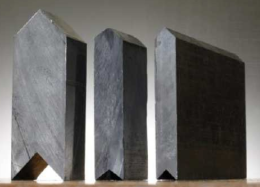
\includegraphics[width=\textwidth]{3DesignPrinciples/34BackgroundRejectionSystem/LeadBricks.png}  
    \caption{Lead bricks.\label{subfig:LeadBricks}}
    \end{subfigure}
    \hfill
    \begin{subfigure}[b]{0.3\textwidth}
    \centering
    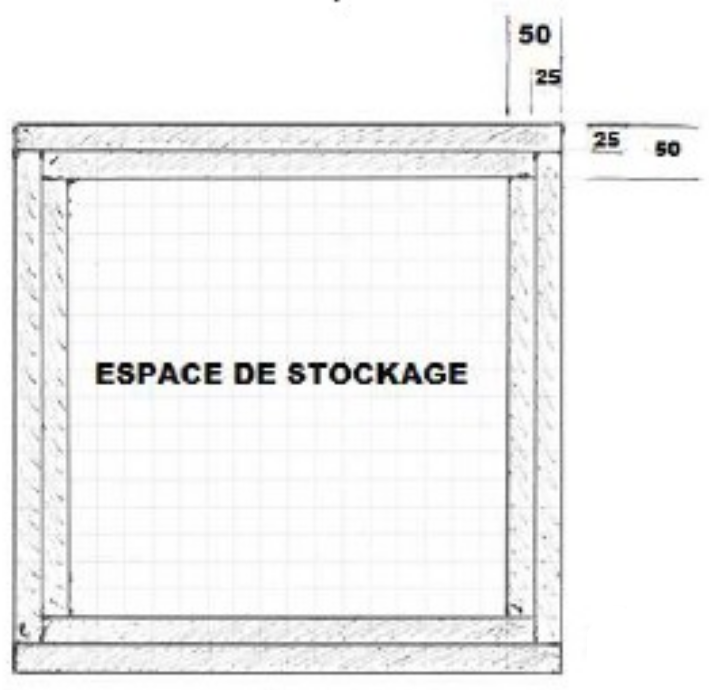
\includegraphics[width=\textwidth]{3DesignPrinciples/34BackgroundRejectionSystem/TwoLayers.png}  
    \caption{Two layers for the lead bricks of the shielding.\label{subfig:TwoLayers}}
    \end{subfigure}
    \hfill
    \begin{subfigure}[b]{0.3\textwidth}
    \centering
    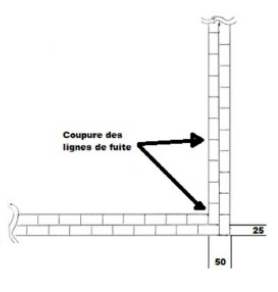
\includegraphics[width=\textwidth]{3DesignPrinciples/34BackgroundRejectionSystem/TwoLayers2.png}  
    \caption{Two layers for the lead bricks of the shielding.\label{subfig:TwoLayers2}}
    \end{subfigure}
 \caption{Lead Bricks and their arrangement in the lead shielding.}
 \label{fig:LeadBricksAndArrangement}
\end{figure}

A special aluminum structure, shown in Figure \ref{fig:AluminiumStructure}, was designed by mechanical engineering department of CENBG to support the total weight of the lead bricks, $2.4$ tons.

\begin{figure}
\centering
    \begin{subfigure}[b]{0.45\textwidth}
    \centering
    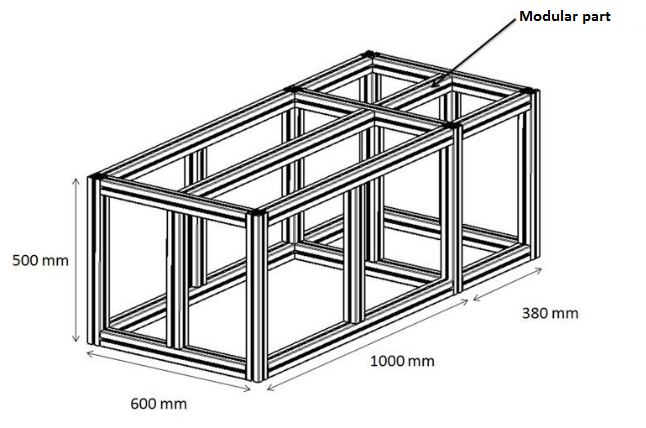
\includegraphics[width=\textwidth]{3DesignPrinciples/34BackgroundRejectionSystem/AluminiumStructureScheme.png}  
    \caption{Aluminium structure scheme.\label{subfig:AluminiumStructureScheme}}
    \end{subfigure}
    \hfill
    \begin{subfigure}[b]{0.4\textwidth}
    \centering
    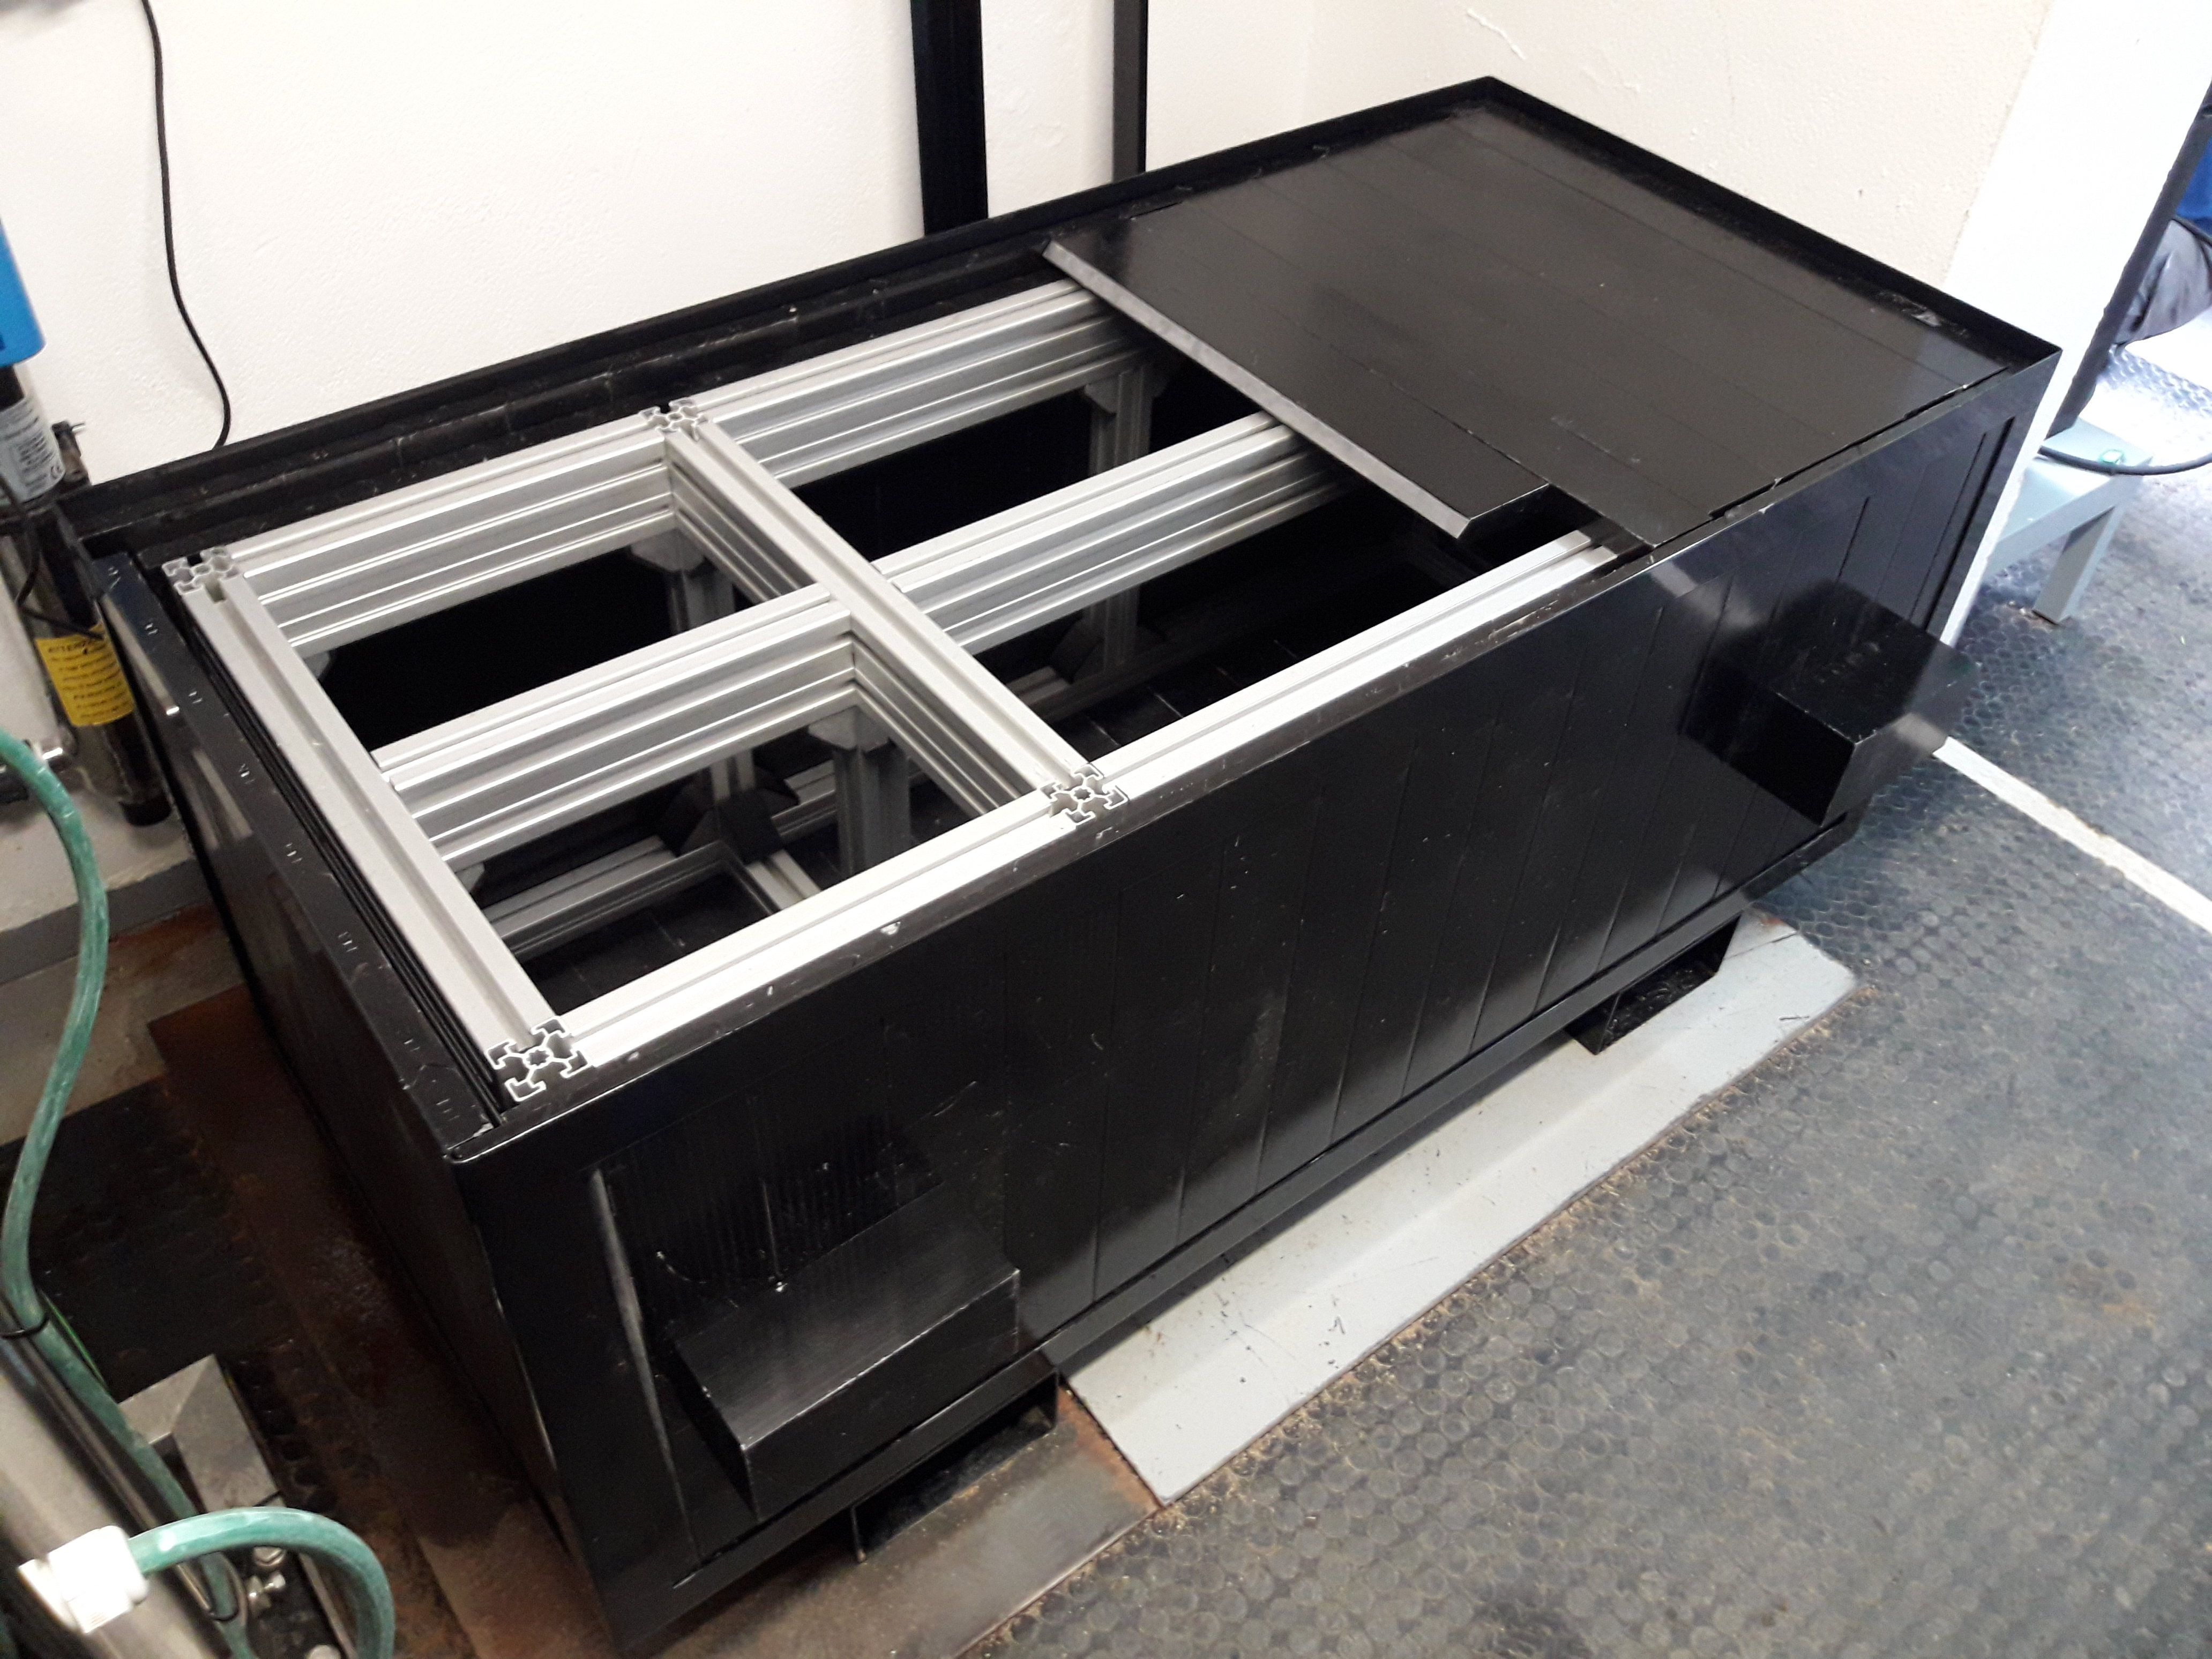
\includegraphics[width=\textwidth]{3DesignPrinciples/34BackgroundRejectionSystem/AluminiumStructure.jpg}  
    \caption{Aluminium structure of TRITIUM monitor.\label{subfig:AluminiumStructure}}
    \end{subfigure}
    \caption{Lead Bricks and their arrangement in the lead shielding.}
 \label{fig:AluminiumStructure}
\end{figure}

The internal room of the lead shielding is divided in two parts, as exhibited in Figure \ref{fig:LeadBricksAndArrangement}. The larger one has internal dimensions of $90.5 \times 41 \times 51~\cm^3$ and is used to place the TRITIUM detector. The smaller one, of dimensions of $33 \times 41 \times 51~\cm^3$, contains the DAQ system. The external dimensions of the lead shielding are $148 \times 60 \times 70~\cm^3$ and a weighs $2.5$ tons.